\section{Comportamiento del amplificador operacional no inversor}

A lo largo de esta sección se procederá a analizar el comportamiento
ideal y real del amplificador operacional \emph{LM324 }conectado como
se muestra en la figura \ref{1_b_1}. Considerando los valores de
los componentes como se observa en la tabla \ref{1_a_t_1}. 

\begin{figure}[H]
\begin{centering}
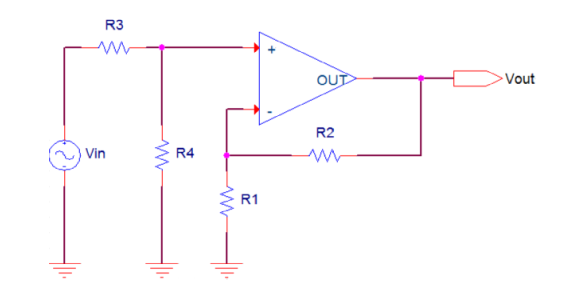
\includegraphics[scale=0.5]{../Ex1/ib/Resources1b/circuit}
\par\end{centering}
\caption{Circuito B}
\label{1_b_1}

\end{figure}

Se implementó en \emph{Altium Designer }como se muestra en las figuras
\ref{1_b_2} y \ref{1_b_3}.

\begin{figure}[H]
\begin{centering}
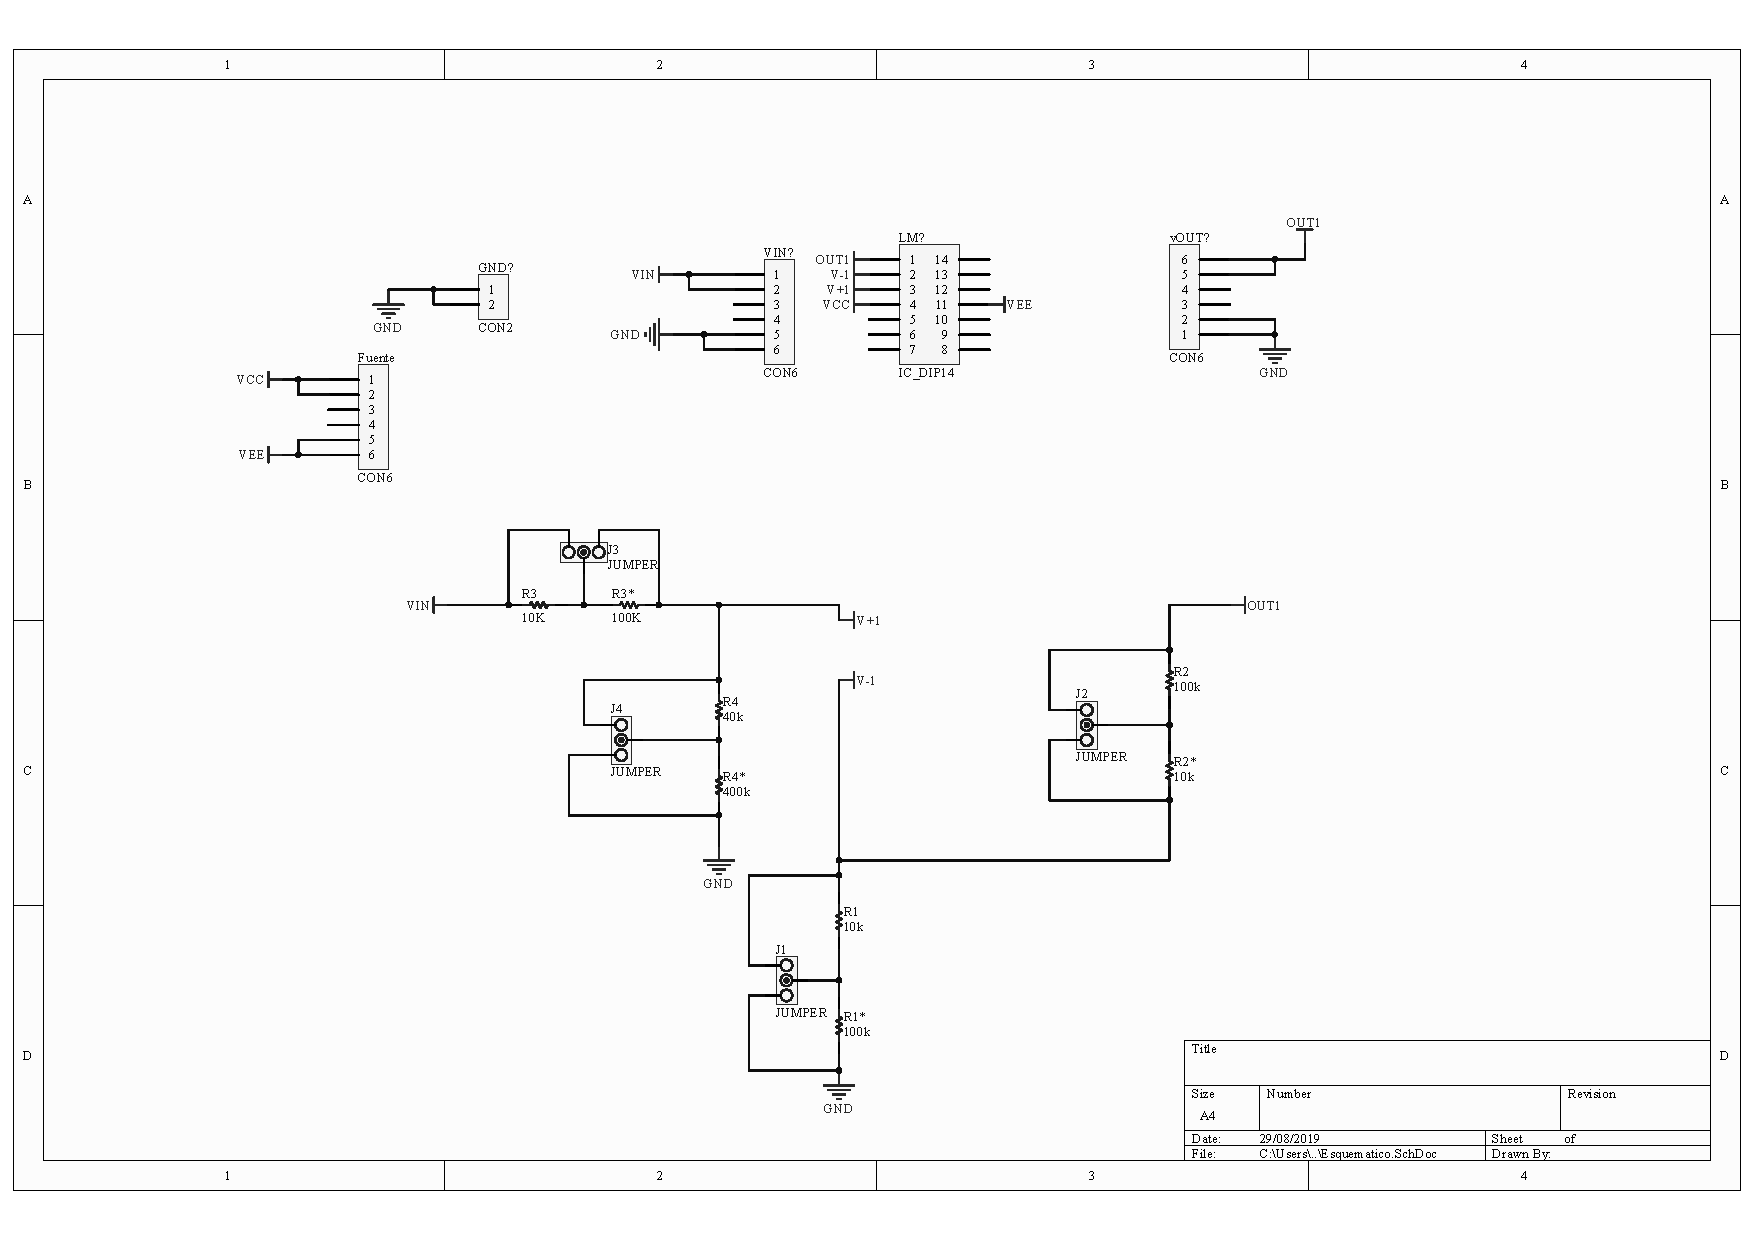
\includegraphics[scale=0.5]{../Ex1/ib/Resources1b/Schematic}
\par\end{centering}
\caption{Esquemático del circuito implementado}
\label{1_b_2}

\end{figure}

\begin{figure}[H]
\begin{centering}
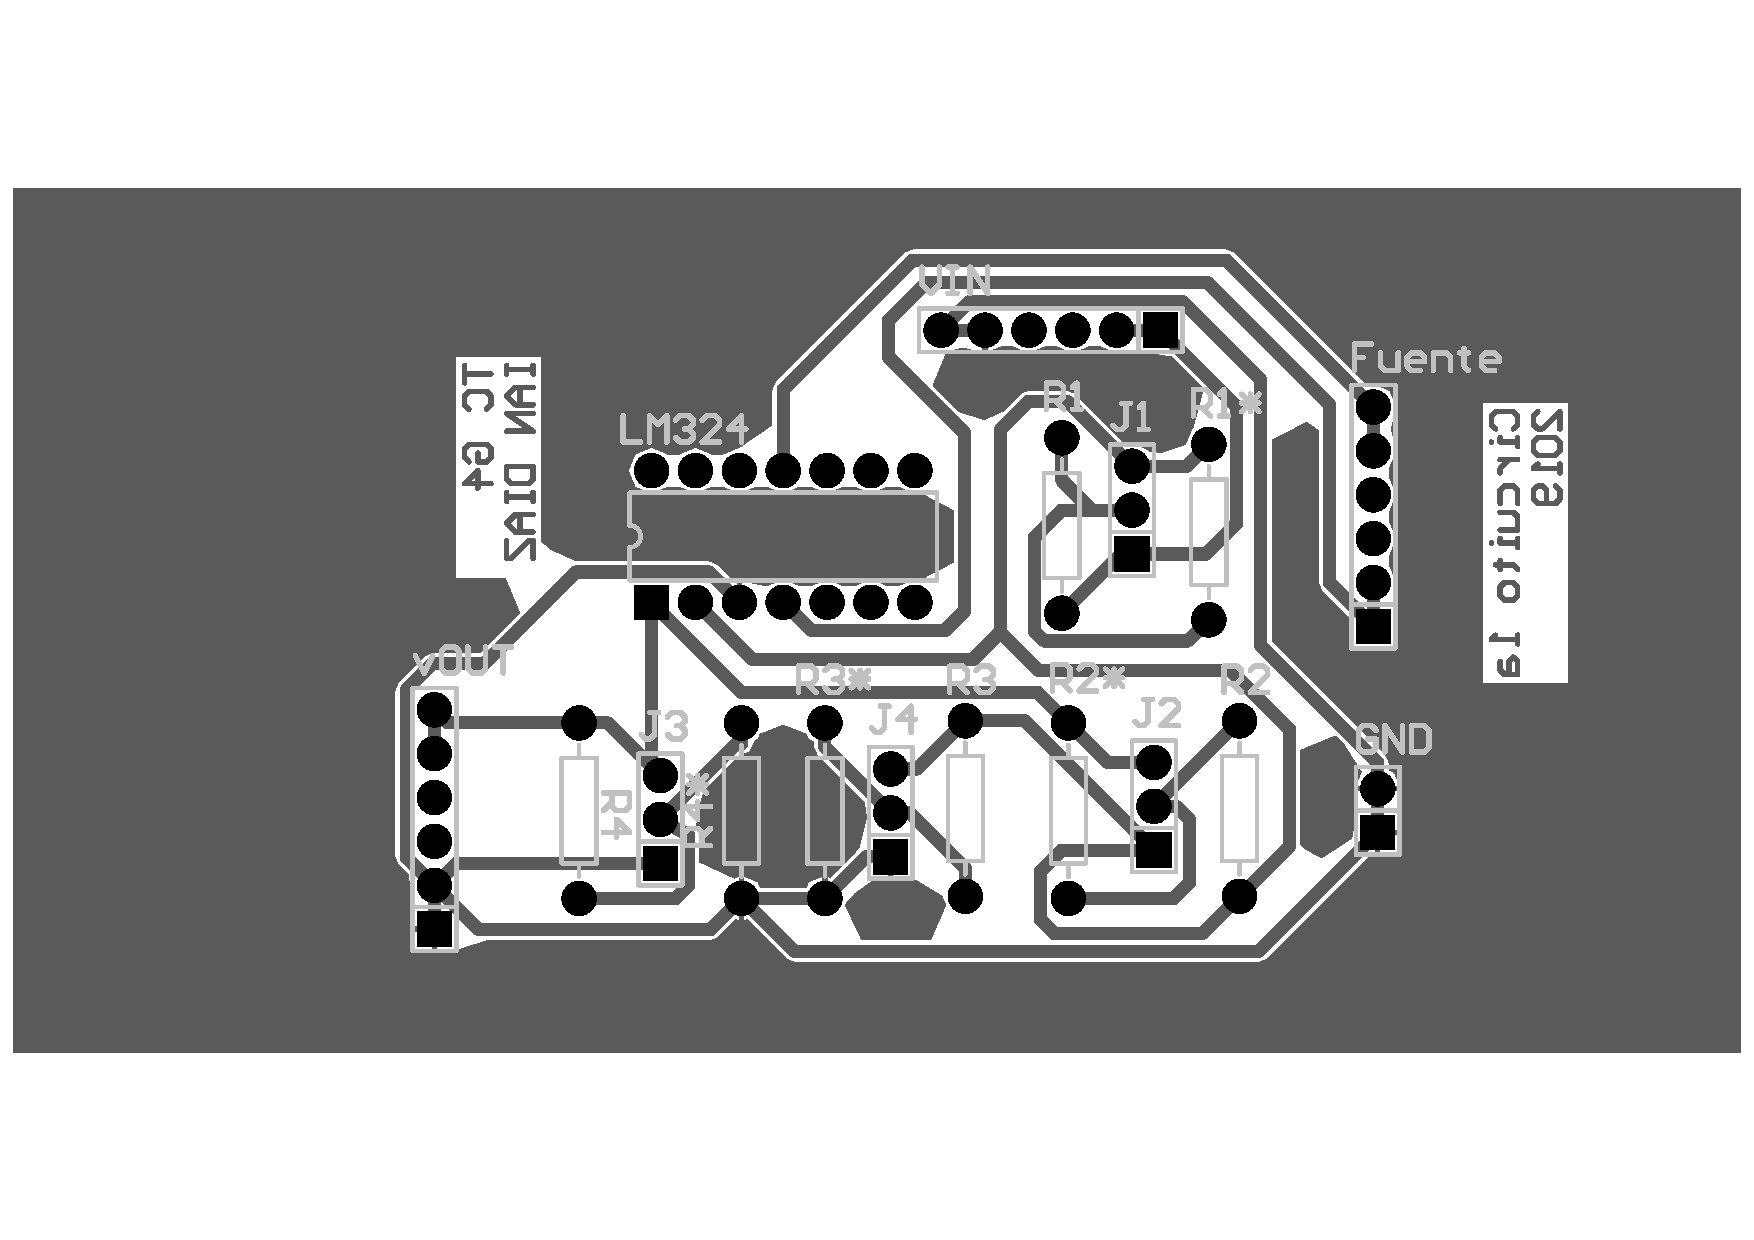
\includegraphics[scale=0.3]{../Ex1/ib/Resources1b/PCB}
\par\end{centering}
\caption{PCB del circuito implementado}
\label{1_b_3}

\end{figure}

\subsection{Análisis de la transferencia}

Comenzando por el análisis ideal, se pidió calcular y graficar la
relación $\frac{V_{out}}{V_{in}}$, esto quiere decir, considerando
$a_{0}$ finito y $A(\omega)$ con polo dominante. Considerando las
ecuaciones descriptas a continuación y operando correctamente, se
llega a que la relación $\frac{V_{out}}{V_{in}}$ está dada por la
ecuación (\ref{eq:1_b_1}).

\[
\left\{ \begin{array}{c}
\frac{V_{i}-V^{+}}{R_{3}}=\frac{V^{+}}{R_{4}}\\
\frac{V_{o}-V^{-}}{R_{2}}=\frac{V^{-}}{R_{1}}\\
V_{o}=A(\omega)(V^{+}-V^{-})
\end{array}\right.
\]

\begin{equation}
H(s)=\frac{R_{4}\omega_{p}a_{0}\left(R_{1}+R_{2}\right)}{\left(R_{3}-R_{4}\right)\left(R_{1}\omega_{p}a_{0}+\left(R_{1}+R_{2}\right)\left(\omega_{p}+s\right)\right)}\label{eq:1_b_1}
\end{equation}

\[
H(s)=\frac{414\times10^{9}}{110\times10^{3}s+47\times10^{9}}\,\,\,Caso\,1
\]

\[
H(s)=\frac{75\times10^{9}}{20\times10^{3}s+47\times10^{9}}\,\,\,Caso\,2
\]

\[
H(s)=\frac{414\times10^{9}}{110\times10^{3}s+471\times10^{9}}\,\,\,Caso\,3
\]

\begin{figure}[H]
\begin{centering}
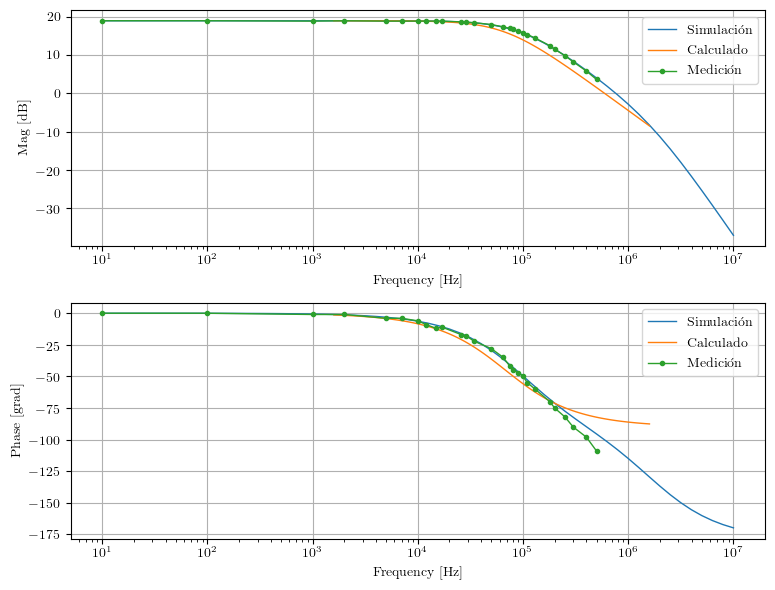
\includegraphics[scale=0.5]{../Ex1/ib/Resources1b/H1b}
\par\end{centering}
\caption{Comportamiento del circuito para el caso 1}
\end{figure}

\begin{figure}[H]
\begin{centering}
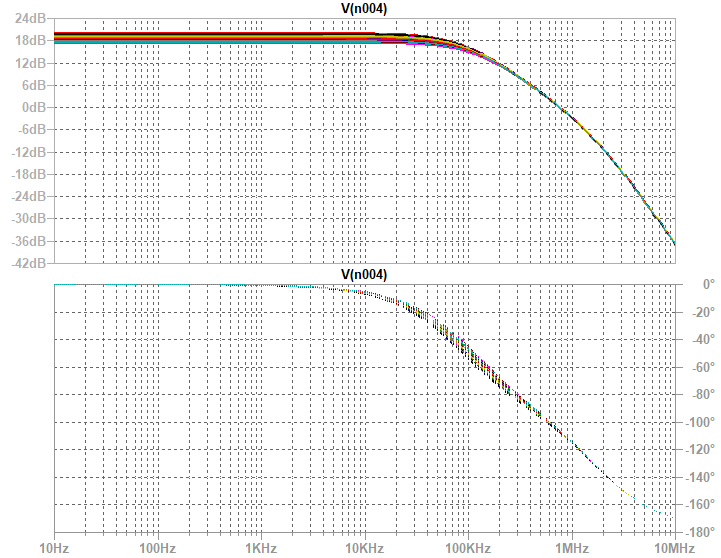
\includegraphics[scale=0.5]{../Ex1/ib/Resources1b/Montecarlo1}
\par\end{centering}
\caption{Análisis Montecarlo del caso 1}
\end{figure}

\begin{figure}[H]
\begin{centering}
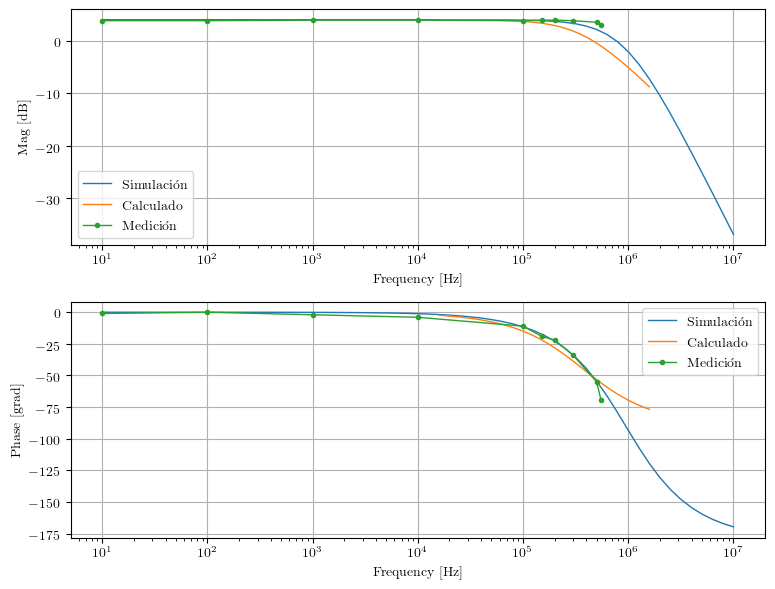
\includegraphics[scale=0.5]{../Ex1/ib/Resources1b/H2b}
\par\end{centering}
\caption{Comportamiento del circuito para el caso 2}
\end{figure}

\begin{figure}[H]
\begin{centering}
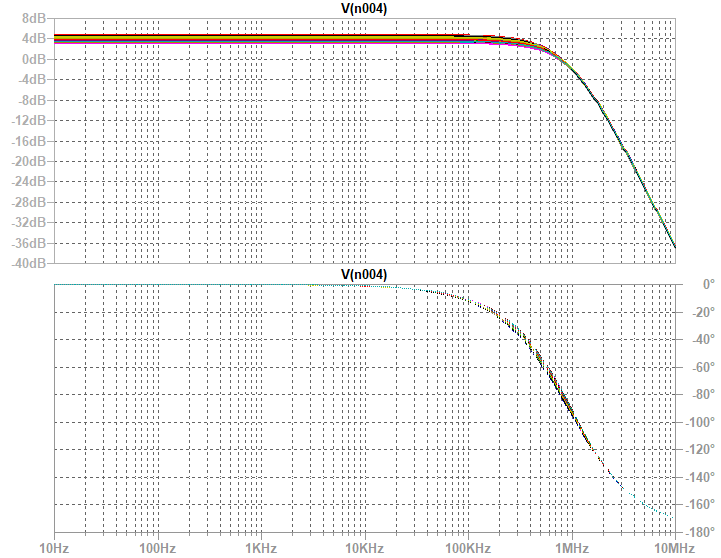
\includegraphics[scale=0.5]{../Ex1/ib/Resources1b/Montecarlo2}
\par\end{centering}
\caption{Análisis Montecarlo del caso 2}
\end{figure}

\begin{figure}[H]
\begin{centering}
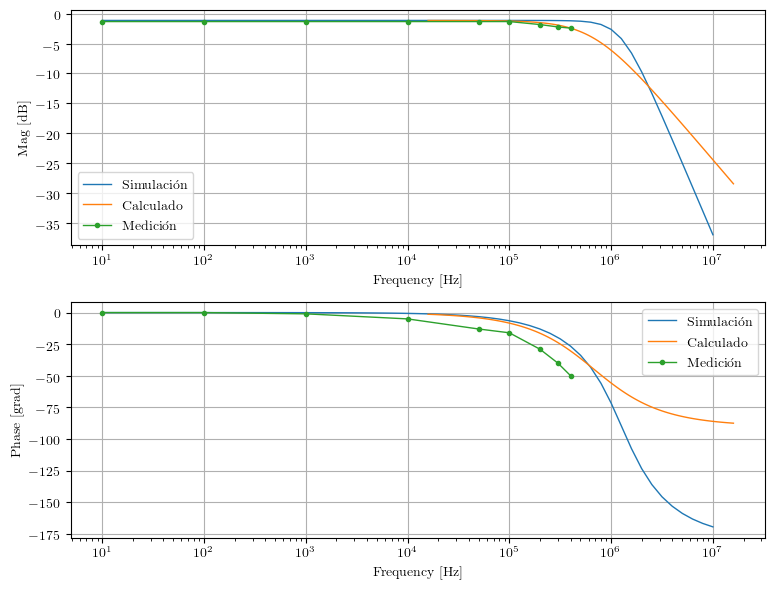
\includegraphics[scale=0.5]{../Ex1/ib/Resources1b/H3b}
\par\end{centering}
\caption{Comportamiento del circuito para el caso 3}
\end{figure}

\begin{figure}[H]
\begin{centering}
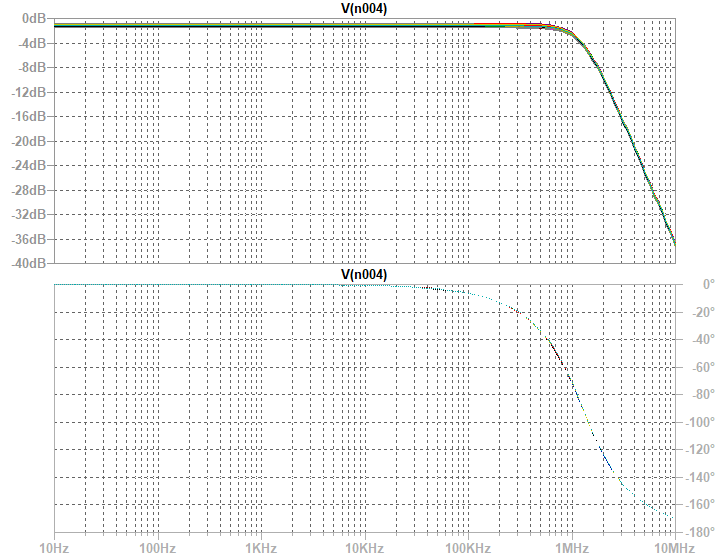
\includegraphics[scale=0.5]{../Ex1/ib/Resources1b/Montecarlo3}
\par\end{centering}
\caption{Análisis Montecarlo del caso 3}
\end{figure}

Como se puede observar, los circuitos siguen dentro de los parámetros
adecuados, y considerando capacidades, inductancias y resistencias
parásitas, las simulaciones y la transferencias calculadas. Las diferencias
entre la transferencia calculada y la simulación se deben a las puntas
de los osciloscopios, que generan polos de $2^{do}$ orden, sumados
a los polos de los capacitores internos a los transistores de juntura
bipolar, que provocan que la pendiente de atenuacion del circuito
se mayor a la calculada, y a su vez, que el cambio de fase no sea
de 90\textdegree , sino de 180\textdegree .

\subsection{Análisis de la impedancia de entrada}

Consecuentemente, se instó a calcular la impedancia de entrada vista
por el generador hacia el circuito. Nuevamente, se utilizo el \emph{Circuit
Solver }creado en Python para calcular las expresiones de las impedancias
de entrada. La ecuación que describe la impedancia de entrada se detalla
en la ecuación (\ref{eq:1_b_2}).

\begin{equation}
Z_{inp}=R_{3}+R_{4}\label{eq:1_b_2}
\end{equation}

Por lo tanto, las impedancias de entrada para cada caso serán:

\[
Z_{inp}=50(k\Omega)\,\,\,Caso\,1
\]

\[
Z_{inp}=50(k\Omega)\,\,\,Caso\,2
\]

\[
Z_{inp}=500(k\Omega)\,\,\,Caso\,3
\]

Teniendo en cuenta estos resultados, y a diferencia de lo visto previamente
en el análisis del circuito inversor, se puede observar como la impedancia
de entrada permanece constante frente a cambios de frecuencia en la
tensión de entrada.

\begin{figure}[H]
\begin{centering}
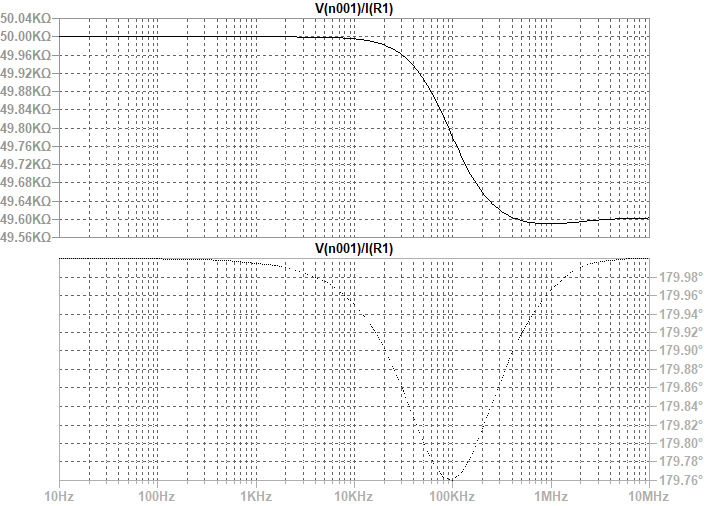
\includegraphics[scale=0.5]{../Ex1/ib/Resources1b/zinp1_sim}
\par\end{centering}
\caption{Simulación de la impedancia de entrada para el caso 1}

\end{figure}

\begin{figure}[H]
\begin{centering}
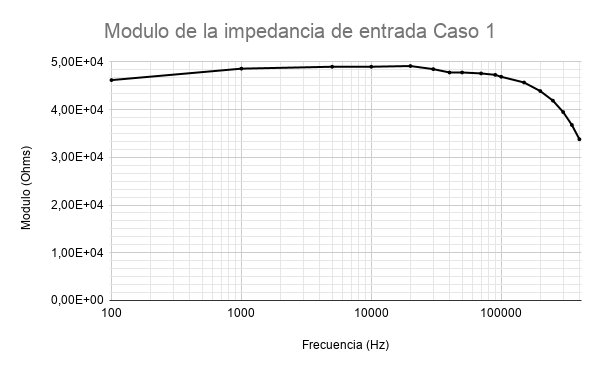
\includegraphics[scale=0.4]{../Ex1/ib/Resources1b/zinp1_m_med}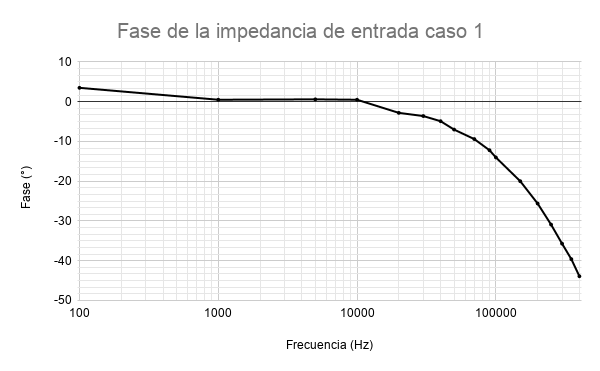
\includegraphics[scale=0.4]{../Ex1/ib/Resources1b/zinp1_p_med}
\par\end{centering}
\caption{Medición de la impedancia de entrada para el caso 1}

\end{figure}

\begin{figure}[H]
\begin{centering}
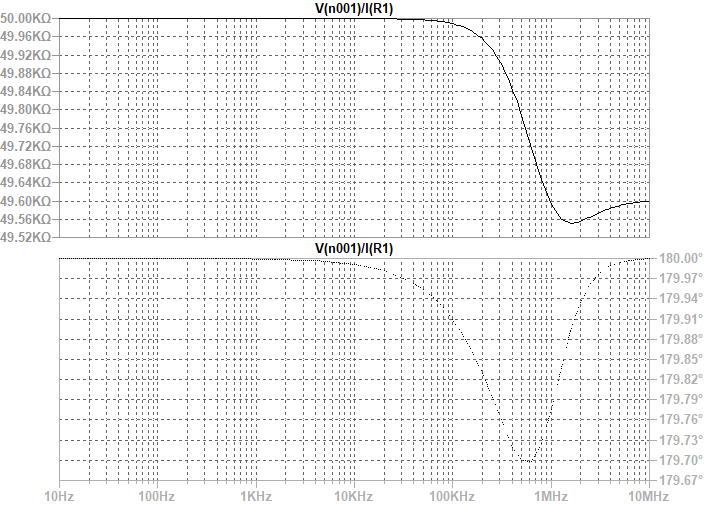
\includegraphics[scale=0.5]{../Ex1/ib/Resources1b/zinp2_sim}
\par\end{centering}
\caption{Simulación de la impedancia de entrada para el caso 2}
\end{figure}

\begin{figure}[H]
\begin{centering}
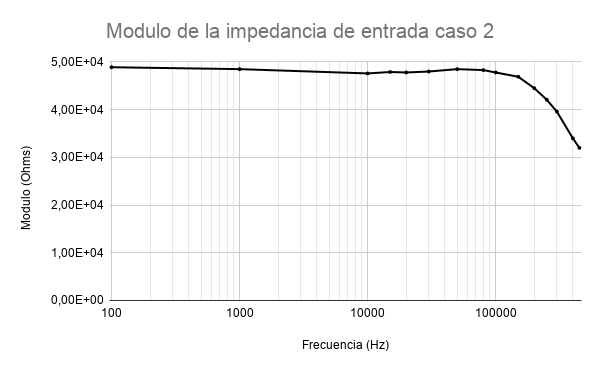
\includegraphics[scale=0.4]{../Ex1/ib/Resources1b/zinp2_m_med}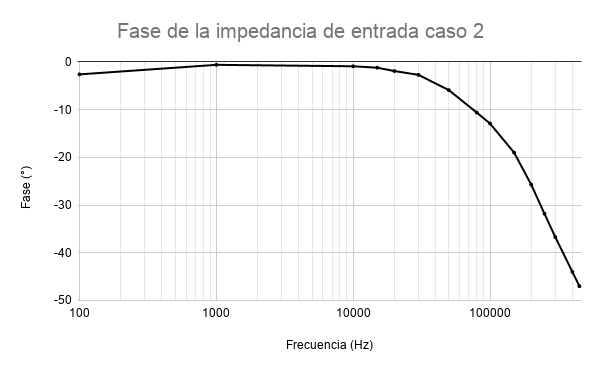
\includegraphics[scale=0.4]{../Ex1/ib/Resources1b/zinp2_p_med}
\par\end{centering}
\caption{Medición de la impedancia de entrada para el caso 2}
\end{figure}

\begin{figure}[H]
\begin{centering}
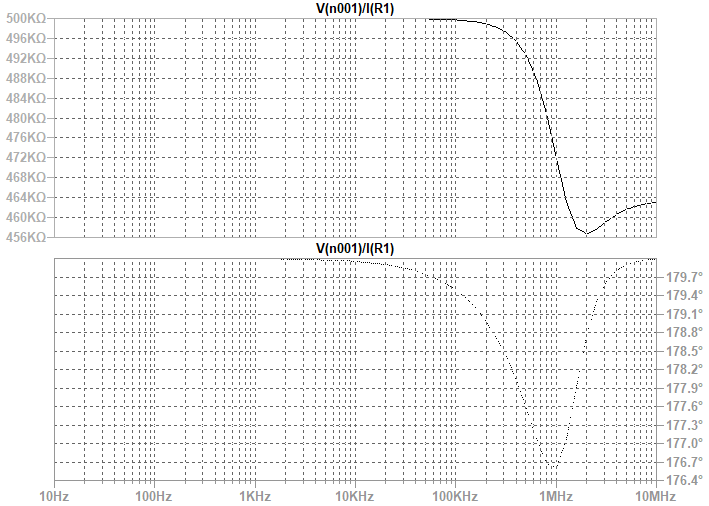
\includegraphics[scale=0.5]{../Ex1/ib/Resources1b/zinp3_sim}
\par\end{centering}
\caption{Simulación de la impedancia de entrada para el caso 3}
\end{figure}

\begin{figure}[H]
\begin{centering}
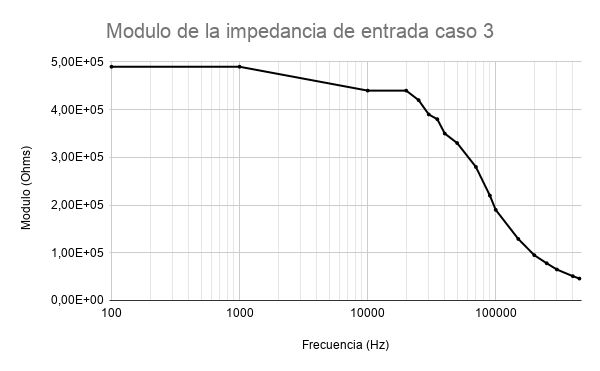
\includegraphics[scale=0.4]{../Ex1/ib/Resources1b/zinp3_m_med}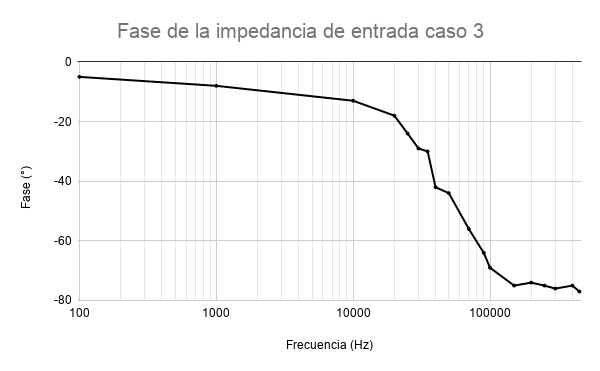
\includegraphics[scale=0.4]{../Ex1/ib/Resources1b/zinp3_p_med}
\par\end{centering}
\caption{Medición de la impedancia de entrada para el caso 3}
\end{figure}

Observando los gráficos de las simulaciones y comparandolos con las
ecuación (\ref{eq:1_b_2}), se puede observar como prácticamente la
impedancia de entrada permanece constante para todas las frecuencias.
El hecho de que la impedancia de entrada tenga una pequeña variación
en módulo y fase en la simulación se debe a que para hacer el análisis
de la impedancia de entrada se consideró el amplificador operacional
ideal, es decir, $R_{id}\longrightarrow\infty$ y $R_{o}\longrightarrow0$
por lo tanto, no se tienen en cuenta el efecto de esas resistencias,
como a su vez sus inductancias y capacidades intrínsecas del amplificador.
Sin embargo, considerando la ecuación propuesta, y observando los
resultados simulados, se puede observar que prácticamente no hay problema
en aproximar la impedancia de entrada como constante en ninguno de
los tres casos (considerando un 10\% de error en el ultimo caso).

Por otro lado, si se analizan las mediciones, se puede ver que para
frecuencias mayores a 10(kHz), el modelo se aleja bastante de los
resultados empíricos. Esto se explica debido a las capacidades parásitas
que se generaron a la hora de medir la impedancia de entrada, que
considerando a $Z_{inp}=R_{3}+R_{4}$ generan un circuito pasabajos
de primer orden, obteniendo así los resultados vistos en las mediciones.
Si se simula el circuito, considerando las capacidades parásitas,
comienza a ser observable el efecto pasabajos que se genera, y se
pone en evidencia los resultados empíricos.

\begin{figure}[H]
\begin{centering}
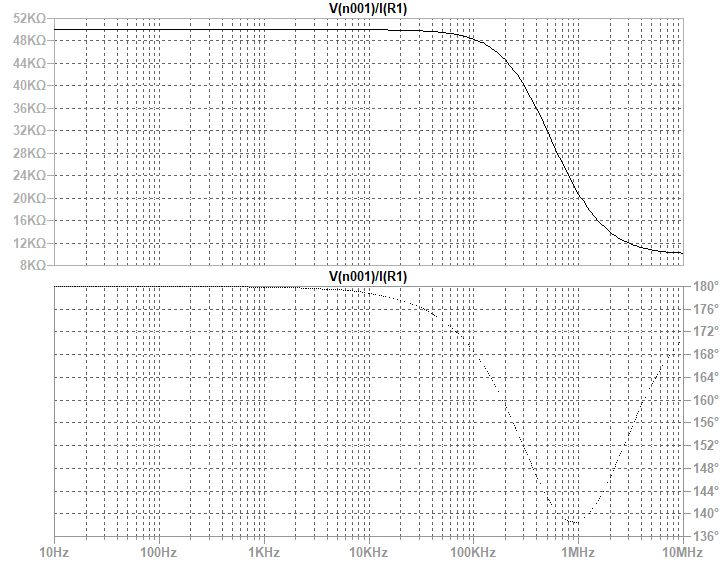
\includegraphics[scale=0.5]{../Ex1/ib/Resources1b/zinp1_sim_para}
\par\end{centering}
\begin{centering}
\caption{Simulación de impedancia de entrada para el caso 1, considerando una
capacidad parásita de 10(pF)}
\par\end{centering}
\end{figure}

\begin{figure}[H]
\begin{centering}
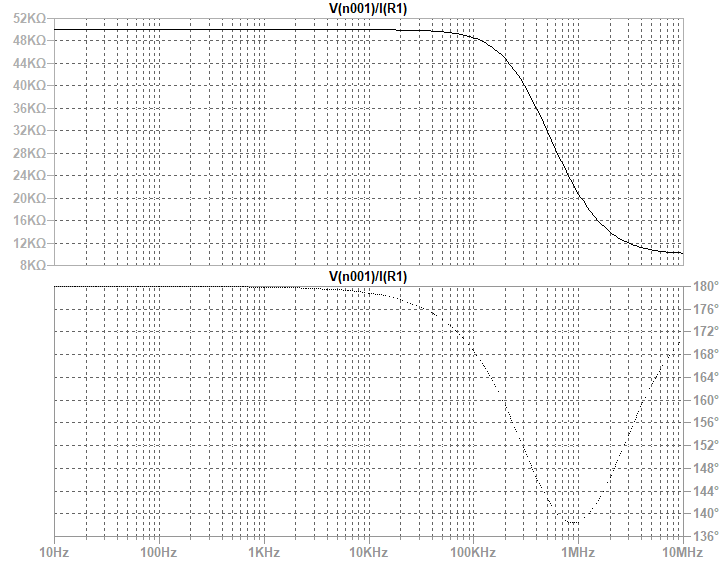
\includegraphics[scale=0.5]{../Ex1/ib/Resources1b/zinp2_sim_para}
\par\end{centering}
\centering{}\caption{Simulación de impedancia de entrada para el caso 2, considerando una
capacidad parásita de 10(pF)}
\end{figure}

\begin{figure}[H]
\begin{centering}
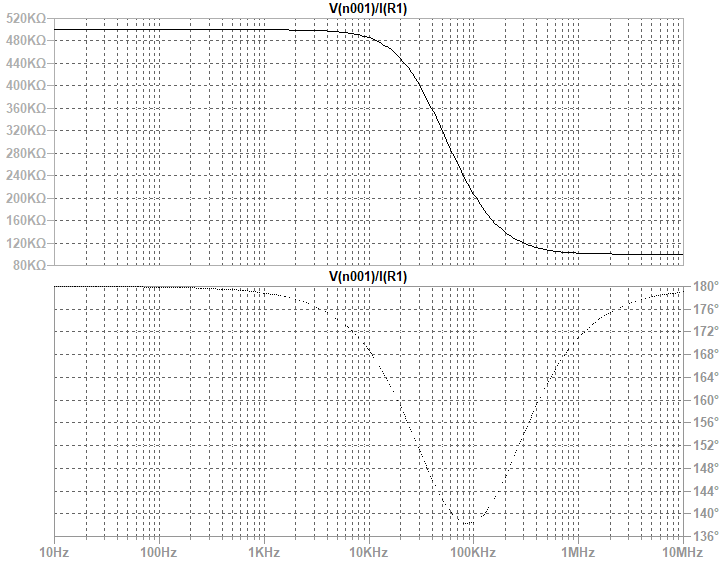
\includegraphics[scale=0.5]{../Ex1/ib/Resources1b/zinp3_sim_para}
\par\end{centering}
\centering{}\caption{Simulación de impedancia de entrada para el caso 3, considerando una
capacidad parásita de 10(pF)}
\end{figure}

\subsection{Análisis de alinealidades}

\subsubsection{Análisis de saturación y polo dominante}

Teniendo en cuenta que la salida del amplificador operacional no podrá
ser en módulo mayor a $V_{cc}$, se calculó, como se explico en la
sección anterior, el máximo valor de la tensión de entrada dependiente
de la frecuencia de entrada para el cual el circuito no satura.

\[
\left|H(f)\right|\times V_{in}=\frac{R_{4}\omega_{p}a_{0}\left(R_{1}+R_{2}\right)}{\left(R_{3}+R_{4}\right)\sqrt{4f^{2}\pi^{2}\left(R_{1}+R_{2}\right)^{2}+\left(R_{1}\omega_{p}a_{0}+\omega_{p}\left(R_{1}+R_{2}\right)\right)^{2}}}\times V_{in}\leq V_{cc}
\]

\[
V_{in}\leq\frac{Vcc\left(R_{3}+R_{4}\right)\sqrt{4\pi^{2}f^{2}\left(R_{1}+R_{2}\right)^{2}+\left(R_{1}\omega_{p}a_{0}+R_{1}\omega_{p}+R_{2}\omega_{p}\right)^{2}}}{R_{4}\omega_{p}a_{0}\left(R_{1}+R_{2}\right)}
\]

\[
V_{in}\leq2.4\cdot10^{-12}Vcc\sqrt{48,4\times10^{9}\pi^{2}f^{2}+2.2\cdot10^{21}}\,\,\,Caso\,1
\]

\[
V_{in}\leq1.3\cdot10^{-11}Vcc\sqrt{1,6\times10^{9}\pi^{2}f^{2}+2.2\cdot10^{21}}\,\,\,Caso\,2
\]

\[
V_{in}\leq2.4\cdot10^{-12}Vcc\sqrt{48,4\times10^{9}\pi^{2}f^{2}+2.2\cdot10^{23}}\,\,\,Caso\,3
\]

Observando estas ecuaciones y graficandolas para cada caso, se puede
ver que en general, para grandes frecuencias, el efecto de saturación
no se hace presente debido al comportamiento pasabajos del circuito
analizado.

\begin{figure}[H]
\begin{centering}
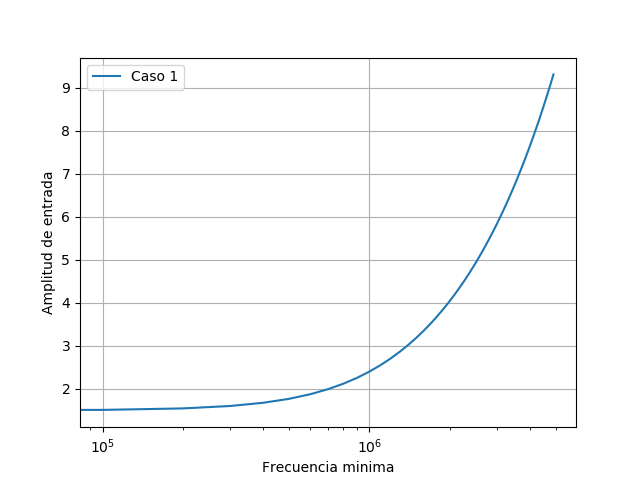
\includegraphics[scale=0.5]{../Ex1/ib/Resources1b/sat1}
\par\end{centering}
\begin{centering}
\caption{Tensión de entrada máxima respecto de la frecuencia de entrada para
que no ocurra saturación en el caso 1}
\par\end{centering}
\end{figure}

\begin{figure}[H]
\begin{centering}
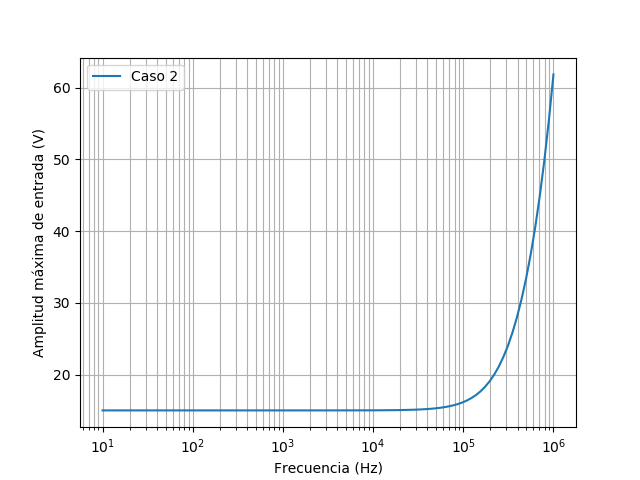
\includegraphics[scale=0.5]{../Ex1/ib/Resources1b/sat2}
\par\end{centering}
\centering{}\caption{Tensión de entrada máxima respecto de la frecuencia de entrada para
que no ocurra saturación en el caso 2}
\end{figure}

\begin{figure}[H]
\begin{centering}
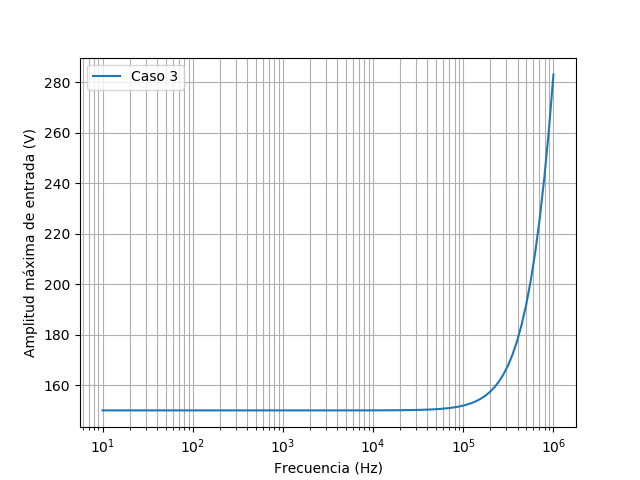
\includegraphics[scale=0.5]{../Ex1/ib/Resources1b/sat3}
\par\end{centering}
\centering{}\caption{Tensión de entrada máxima respecto de la frecuencia de entrada para
que no ocurra saturación en el caso 3}
\end{figure}

\begin{figure}[H]
\begin{centering}
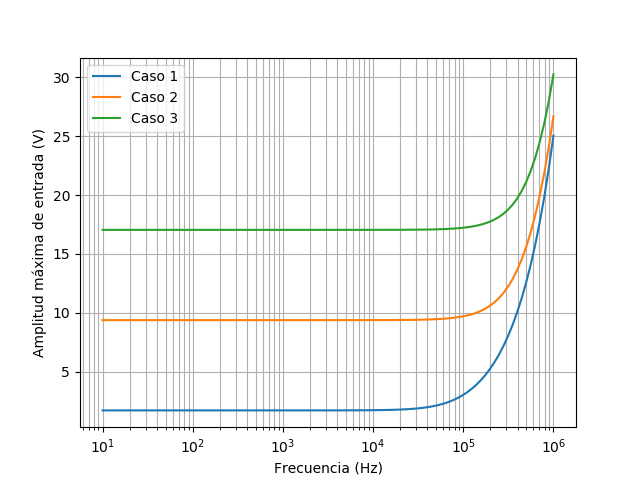
\includegraphics[scale=0.5]{../Ex1/ib/Resources1b/sat123}
\par\end{centering}
\centering{}\caption{Tensión de entrada máxima respecto de la frecuencia de entrada para
que no ocurra saturación}
\end{figure}

\subsubsection{Análisis de \emph{Slew Rate}}

Por otro lado, se analizó el efecto \emph{Slew Rate }de la misma manera
que se lo hizo en la seccion anterior, es decir, $\frac{\partial V_{out}}{\partial t}\leq SR$,
por lo tanto, tenemos que, $v_{in}(t)=V_{p}sin(2\pi ft)$, por ende,
$V_{out}(t)=\left|H(f)\right|V_{p}2\pi f\,cos(2\pi ft+\phi(f))$.
A su vez, el coseno siempre es menor a 1, por ende:

\[
\frac{\partial V_{out}}{\partial t}\leq\left|H(f)\right|V_{p}2\pi f\leq SR
\]

\begin{equation}
\Rightarrow V_{p}\leq\frac{SR}{\left|H(f)\right|f2\pi}\label{eq:1_b_asd}
\end{equation}

Reemplazando en la inecuación (\ref{eq:1_b_asd}), se tiene que;

\[
V_{in}\leq\frac{SR\left(R_{3}+R_{4}\right)\sqrt{4\pi^{2}f^{2}\left(R_{1}+R_{2}\right)^{2}+\left(R_{1}\omega_{p}a_{0}+R_{1}\omega_{p}+R_{2}\omega_{p}\right)^{2}}}{2\pi R_{4}\omega_{p}a_{0}f\left(R_{1}+R_{2}\right)}
\]

\[
V_{in}\leq\frac{1.2\times10^{-12}SR\sqrt{48.2\times10^{9}\pi^{2}f^{2}+2.2\times10^{21}}}{\pi f}\,\,\,Caso\,1
\]

\[
V_{in}\leq\frac{6.6\times10^{-12}SR\sqrt{16\times10^{9}\pi f^{2}+2.2\times10^{21}}}{\pi f}\,\,\,Caso\,2
\]

\[
V_{in}\leq\frac{1.2\times10^{-12}SR\sqrt{48,4\times10^{9}\pi^{2}f^{2}+2.2\times10^{23}}}{\pi f}\,\,\,Caso\,3
\]

Ahora reemplazando para cada caso $SR=0,55836\left(\frac{V}{\mu s}\right)$
(como fue calculado en la sección anterior para el LM324), y se grafica
la amplitud de entrada máxima frente a la frecuencia de entrada, nos
quedan las Figuras \ref{1_b_23}, \ref{1_b_24}, \ref{1_b_25} y \ref{1_b_26}.

\begin{figure}[H]
\begin{centering}
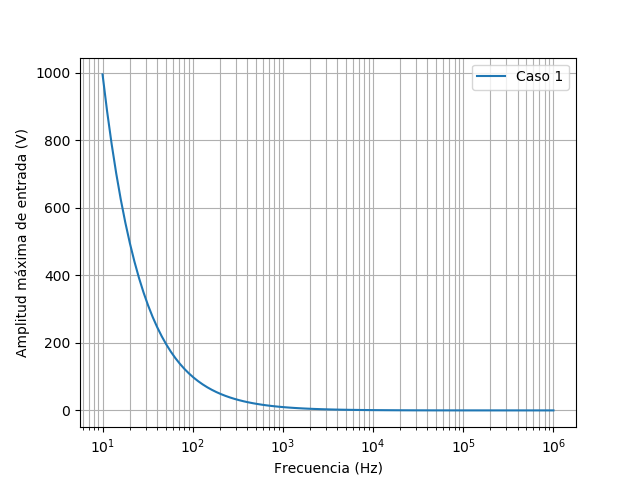
\includegraphics[scale=0.5]{../Ex1/ib/Resources1b/slewRate1}
\par\end{centering}
\centering{}\caption{Tensión de entrada máxima respecto de la frecuencia de entrada para
que no ocurra el efecto de \emph{Slew Rate} en el caso 1}
\label{1_b_23}
\end{figure}

\begin{figure}[H]
\begin{centering}
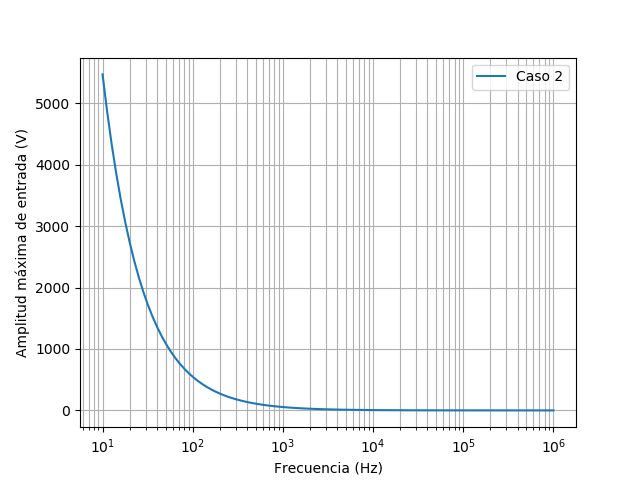
\includegraphics[scale=0.5]{../Ex1/ib/Resources1b/slewRate2}
\par\end{centering}
\centering{}\caption{Tensión de entrada máxima respecto de la frecuencia de entrada para
que no ocurra el efecto de \emph{Slew Rate} en el caso 2}
\label{1_b_24}
\end{figure}

\begin{figure}[H]
\begin{centering}
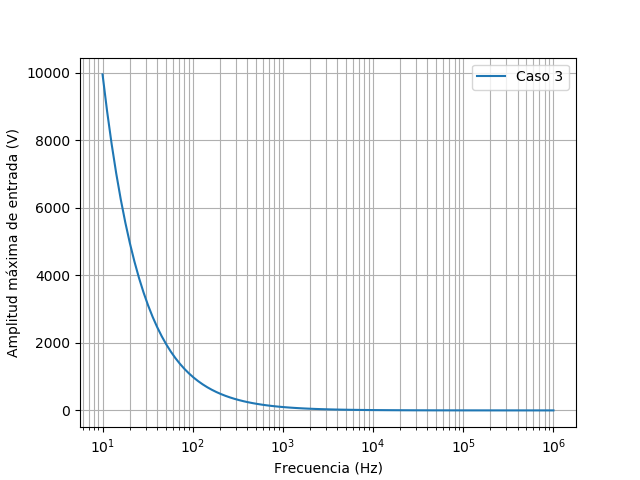
\includegraphics[scale=0.5]{../Ex1/ib/Resources1b/slewRate3}
\par\end{centering}
\centering{}\caption{Tensión de entrada máxima respecto de la frecuencia de entrada para
que no ocurra el efecto de \emph{Slew Rate} en el caso 3}
\label{1_b_25}
\end{figure}

\begin{figure}[H]
\begin{centering}
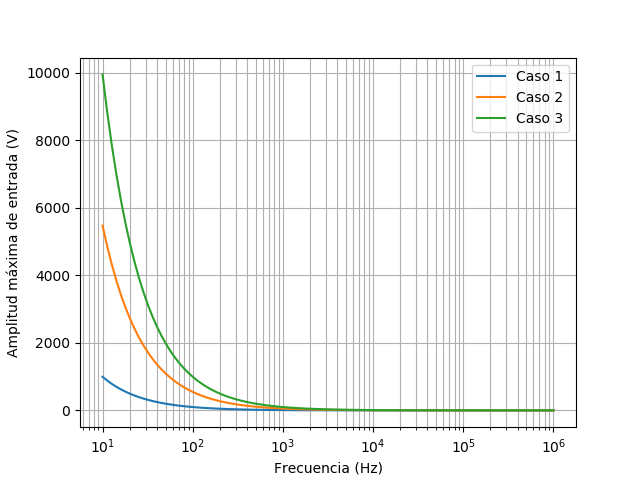
\includegraphics[scale=0.5]{../Ex1/ib/Resources1b/slewRate123}
\par\end{centering}
\centering{}\caption{Tensión de entrada máxima respecto de la frecuencia de entrada para
que no ocurra el efecto de \emph{Slew Rate}}
\label{1_b_26}
\end{figure}

\subsubsection{Conclusiones}

Por último, si se tiene en cuenta los efectos alinealies del \emph{Slew
Rate, }saturación y \emph{Crossover Distortion} (el último explicado
en la sección anterior), pueden ser armadas unas figuras mostradas
a continuación que muestran la máxima amplitud de una señal de entrada
al circuito para cada caso, para que no se encuentren efectos alineales
indeseados en las mediciones. Estas son las figuras \ref{1_b_27},
\ref{1_b_28}, \ref{1_b_29} y \ref{1_b_30}.

\begin{figure}[H]
\begin{centering}
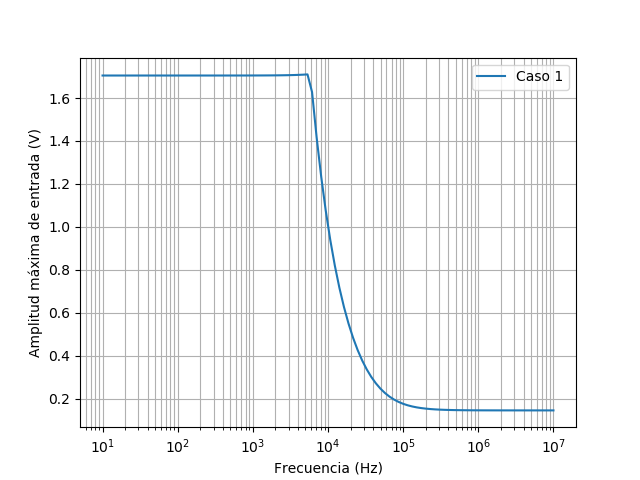
\includegraphics[scale=0.5]{../Ex1/ib/Resources1b/AmplMaxVsFreq1}
\par\end{centering}
\caption{Tensión máxima de entrada para que no ocurran alinealidades en el
caso 1}
\label{1_b_27}

\end{figure}

\begin{figure}[H]
\begin{centering}
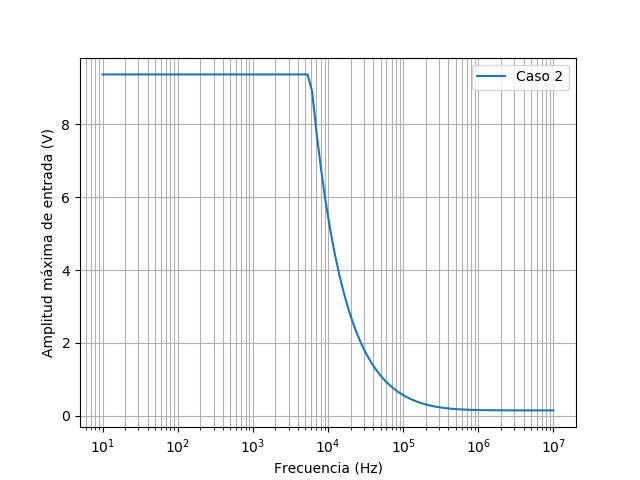
\includegraphics[scale=0.5]{../Ex1/ib/Resources1b/AmplMaxVsFreq2}
\par\end{centering}
\caption{Tensión máxima de entrada para que no ocurran alinealidades en el
caso 2}
\label{1_b_28}
\end{figure}

\begin{figure}[H]
\begin{centering}
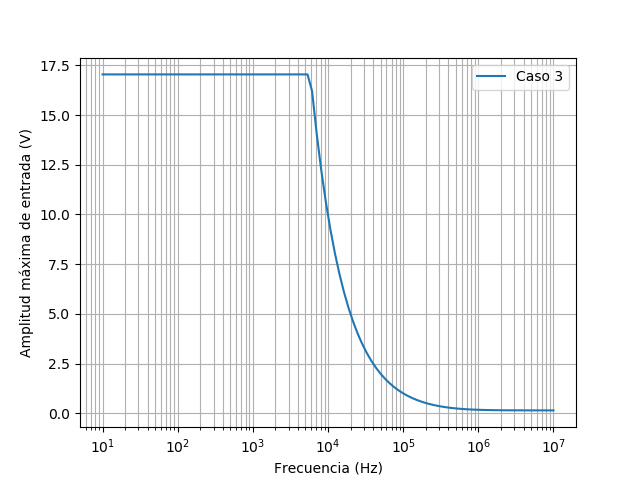
\includegraphics[scale=0.5]{../Ex1/ib/Resources1b/AmplMaxVsFreq3}
\par\end{centering}
\caption{Tensión máxima de entrada para que no ocurran alinealidades en el
caso 3}
\label{1_b_29}
\end{figure}

\begin{figure}[H]
\begin{centering}
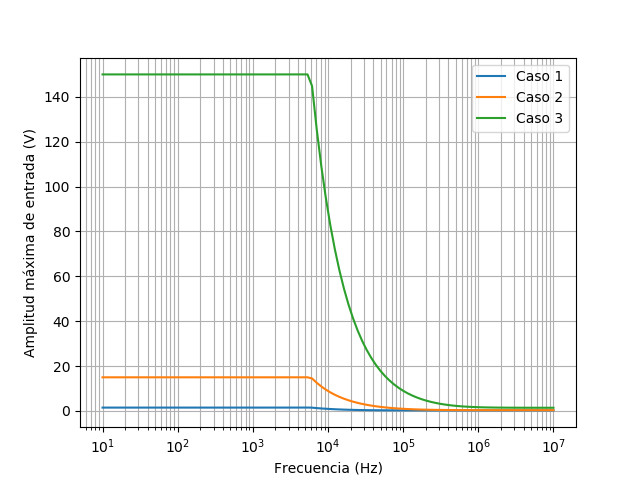
\includegraphics[scale=0.5]{../Ex1/ib/Resources1b/AmplMaxVsFreq123}
\par\end{centering}
\caption{Tensión máxima de entrada para que no ocurran alinealidades}
\label{1_b_30}
\end{figure}

\subsection{Análisis del DC \emph{Sweep}}

A continuación se procede a realizar un DC \emph{Sweep} para cada
caso del circuito, los resultados se muestran a continuación.

\begin{figure}[H]
\begin{centering}
\includegraphics[scale=0.3]{\string"../Ex1/ib/Resources1b/DC Sweep1_sim\string".png}\includegraphics[scale=0.3]{\string"../Ex1/ib/Resources1b/DC Sweep1_med\string".png}
\par\end{centering}
\caption{DC \emph{Sweep} caso 1}
\end{figure}

\begin{figure}[H]
\begin{centering}
\includegraphics[scale=0.3]{\string"../Ex1/ib/Resources1b/DC Sweep2_sim\string".png}\includegraphics[scale=0.3]{\string"../Ex1/ib/Resources1b/DC Sweep2_med\string".png}
\par\end{centering}
\caption{DC \emph{Sweep} caso 2}
\end{figure}

\begin{figure}[H]
\begin{centering}
\includegraphics[scale=0.3]{\string"../Ex1/ib/Resources1b/DC Sweep3_sim\string".png}\includegraphics[scale=0.3]{\string"../Ex1/ib/Resources1b/DC Sweep3_med\string".png}
\par\end{centering}
\caption{DC \emph{Sweep} caso 3}
\end{figure}

Como se puede observar no hay grandes diferencias entre lo simulado
y lo medido.

\section{Conclusiones}

Es determinante tener en cuenta las alinealidades que provoca un amplificador
operacional, ya sea por saturación, \emph{Slew Rate }o \emph{Crossover
Distortion, }ya que es muy importante para proceder a hacer mediciones
sobre los mismos. Estas alinealidades afectan en gran medida el comportamiento
del amplificador operacional, por lo tanto, si no se las tiene en
cuenta, es altamente probable que se cometan errores en mediciones
y resultados esperados.

Sumado a esto, es muy importante tener en cuenta los efectos de los
instrumentos de medición, ya sea osciloscopios, multimetros, analizadores
de impedancias, etc. ya que las capacidades, inductancias y resistencias
parásitas afectan en gran medida el comportamiento de nuestro circuito.

Por último, se pudo observar que a un mismo \emph{Gain Bandwidth Product
}(GBP), podemos cambiar el circuito para que trabaje más idealmente
a altas frecuencias. Es decir que para un caso A con ganancia $\beta$,
y una frecuencia de corte $f_{0}$, y un caso B con ganancia $\beta^{'}$
y una frecuencia de corte $f_{0}^{'}$ , se tiene que $\beta^{'}\leq\beta$
y $f_{0}\leq f_{0}^{'}$, por lo tanto, se podrá en el caso B trabajar
idealmente a mayores frecuencias, pero con menos ganancia, y por el
contrario, en el caso A se trabajará con mas ganancia pero a menores
frecuencias.

Teniendo en cuenta los factores anteriores, si se quiere trabajar
con señales cuadradas de $1V_{pp}$ de frecuencia variante entre $0.3(MHz)\,a\,2(MHz)$,
sera imposible utilizar un LM324 para realizar dicha tarea, ya que
para el GBP dado y el $a_{vol}$ del datasheet, a esas frecuencias,
el amplificador no podrá operar debido al ruido ambiente y al \emph{Slew
Rate. }Una buena opción para realizar una tarea como esta, puede ser
el amplificador operacional TL082, que posee un GBP lo suficientemente
grande como para poder operar en ese rango de frecuencias y un \emph{Slew
Rate }de aproximadamente $13\left(\frac{V}{\mu s}\right)$.

Otra opción podria ser el LM833, ya que posee un valor de $SR=7\left(\frac{V}{\mu s}\right)$
y un $GBP=15(MHz)$. Por ultimo, el amplificador opercaional TL084
es otra buena opcion ya que $SR=13\left(\frac{V}{\mu s}\right)$ y
$GBP=3(MHz)$
